\section{Neuromorphic Engineering}

Neuromorphic computing is a computational paradigm designed to emulate the architecture and behavior of biological nervous systems, such as the human brain. In recent years, the use of \glspl{ann} has surged; however, neuromorphic computing is increasingly gaining attention in the scientific community as a more efficient and promising alternative \cite{Pritchard2023}.

Unlike traditional models that process information sequentially and continuously, neuromorphic computing operates on asynchronous events. In this approach, signals known as ``spikes'' are generated only when a change occurs \cite{Wu2024}.

The core elements of neuromorphic computing are spiking neurons, which collectively form \glspl{snn}. Each neuron processes spikes independently and remains inactive in the absence of input. This event-driven method represents a significant departure from conventional ANNs, which continuously process input signals. By emulating the brain's mechanisms, neuromorphic computing can enhance efficiency and potentially increase computational power for specific tasks \cite{Wu2024}.

However, implementing these models is not without challenges. Hardware limitations, in particular, pose significant obstacles and must be carefully considered to fully leverage the advantages offered by neuromorphic technologies \cite{Pritchard2023}.

\subsection{Spiking Neural Networks.}

%Over the last ten years, deep neural networks have demonstrated outstanding performance across many fields such as language understanding and image recognition. Nonetheless, these models are extremely demanding in terms of resources, requiring vast amounts of energy, large datasets, and substantial computational power the energy consumption of AI data centers is projected to reach 22 billion kWh by 2025 due to increasing model complexity~\cite{tuml2025energy}. For instance, training a large-scale language model like GPT-3, which contains 175 billion parameters, is associated with an energy usage estimated around 190,000 kWh~\cite{brown2020gpt3}. Between 2012 and 2019, the energy demand for training such models increased by roughly a factor of ten, raising concerns about the environmental and economic sustainability of %current AI methods~\cite{delrey2023energy}.

Over the last decade, deep neural networks have achieved remarkable results across various fields including language understanding and image recognition. However, these advances come with substantial resource demands: modern AI models require large datasets, considerable computational power, and significant energy consumption. For example, training large-scale language models such as GPT-3, which contains 175 billion parameters, has been estimated to consume around 190,000 kWh of energy~\cite{brown2020gpt3}. The overall energy consumption of AI data centers is projected to reach 22 billion kWh by 2025, driven primarily by increasing model complexity and the computational intensity of training procedures~\cite{tuml2025energy}. Between 2012 and 2019, the energy required to train state-of-the-art models increased nearly tenfold, raising significant concerns about the environmental and economic sustainability of current AI development practices~\cite{delrey2023energy}.

It is important to distinguish between the energy costs associated with training and those related to inference. Training represents the one-time, upfront energy investment required to develop a model, often consuming vast resources during this phase. Inference, on the other hand, corresponds to the energy expended every time the trained model is deployed to perform tasks such as understanding language, recognizing images, or making decisions in autonomous systems. In many real-world scenarios, particularly those involving large-scale or real-time applications, the cumulative energy consumption during inference can surpass that of training. Therefore, while training energy highlights the environmental footprint of developing AI models, inference energy is a critical metric for assessing their operational efficiency and sustainability in practical deployment contexts.

In a strong contrast, the human brain achieves remarkable computational efficiency by operating with only about 10 to 20 watts while processing complex sensory information ~\cite{muir2025road}. Neuromorphic engineering strives to close this efficiency gap by designing systems inspired by the brain’s organization and function.

The essential components of neuromorphic technology consist of:
\begin{itemize}
    \item \textbf{Neuromorphic sensors}, which detect only changes in input signals rather than continuously sampling, enabling much more efficient data capture~\cite{chicca2025neuromorphic}.
    \item \textbf{Neuromorphic algorithms}, particularly \glspl{snn}, which process information with discrete events or spikes, as shown in Figure \ref{fig:neuro}, mimicking the brain’s temporal coding and typically consuming far less energy than conventional artificial neural networks~\cite{yan2024reconsidering}.
    \item \textbf{Neuromorphic hardware}, specialized computing architectures that implement SNNs and brain-inspired computation, utilizing emerging device technologies such as memristors to improve speed and energy efficiency~\cite{shi2025fully}.
\end{itemize}

A central objective is to integrate the proven effectiveness of artificial neural networks with the energy-saving capabilities of spiking networks. Advances have shown that neuromorphic models running on dedicated platforms can significantly reduce energy consumption and inference latency while maintaining competitive accuracy~\cite{xu2024stcsnn}.

This evolution in computing paradigms is especially critical for applications that require real-time processing under stringent power constraints, including autonomous machines, wearable devices, and brain-machine interfaces~\cite{wang2025energy}.


\begin{figure}[ht]
    \centering
    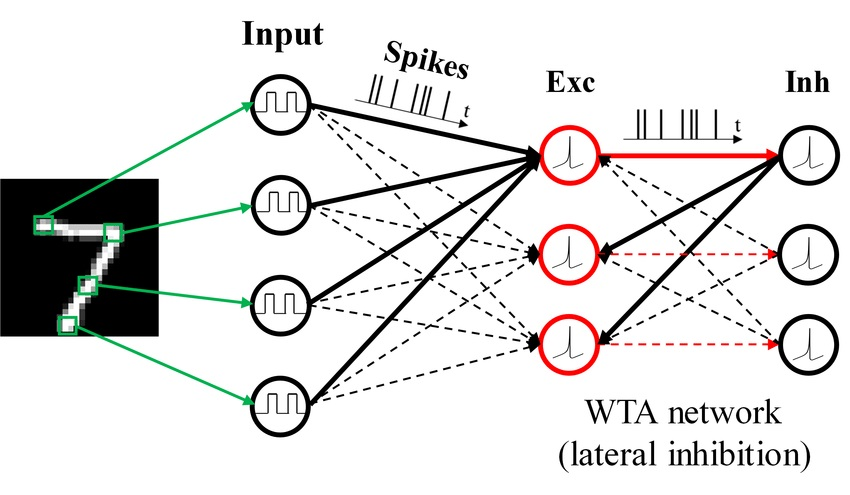
\includegraphics[width=0.8\textwidth]{chap2/figure/snn.jpg}
    \caption{Visual explaination of Neuromorphic algorithm }\cite{arxiv_snn_2510}
    \label{fig:neuro}
\end{figure}


\subsection{Biological Neurons and Their Structure.}

Biological neurons are the elementary signaling units within the nervous systems of animals and humans, forming complex networks capable of adaptive computation. Neurons transmit information primarily via discrete electrical impulses, called spikes or action potentials, facilitating communication between cells and throughout neural circuits \cite{jeon2023distinctive, pircher2021structure}.

A typical neuron consists of several key structural components: dendrites, the soma, axon, and axon terminals. These elements underpin both signal integration and communication within neural circuits \cite{pircher2021structure}.

\begin{itemize}
    \item \textbf{Dendrites}: Dendrites are highly branched projections that receive chemical or electrical signals from other neurons. The morphology and density of dendritic branching modulate a neuron's integration properties and play a pivotal role in the spatial and temporal summation of inputs \cite{pircher2021structure, chung2021neural}.

    \item \textbf{Soma (Cell Body)}: The soma integrates incoming synaptic signals from the dendrites and determines whether the total input surpasses a critical threshold to generate an action potential. The dynamic interplay of excitatory and inhibitory signals shapes the membrane potential and output response \cite{jeon2023distinctive, ma2023mapping}.

    \item \textbf{Axon}: The axon is a long, slender projection that carries the action potential from the cell body to distant targets. Axonal conduction properties affect both the spatial reach and timing of neural signals \cite{pircher2021structure, jeon2023distinctive}.

    \item \textbf{Axon Terminals and Synapses}: Axonal terminals form synapses—the junctions across which signals are transmitted to adjacent neurons or effector cells, commonly using neurotransmitters. The structure, distribution, and plasticity of synapses are essential for learning and adaptation in neural circuits \cite{jeon2023distinctive, lyu2024quantum, chung2021neural}.
\end{itemize}

Neural learning and plasticity are mediated by activity-dependent changes in synaptic strength, enabling adaptive behavior and experience-dependent circuit refinement \cite{chung2021neural}. Modern computational models inspired by these principles offer interpretable and efficient representations of neural processing \cite{ma2023mapping}.

\begin{figure}[ht]
    \centering
    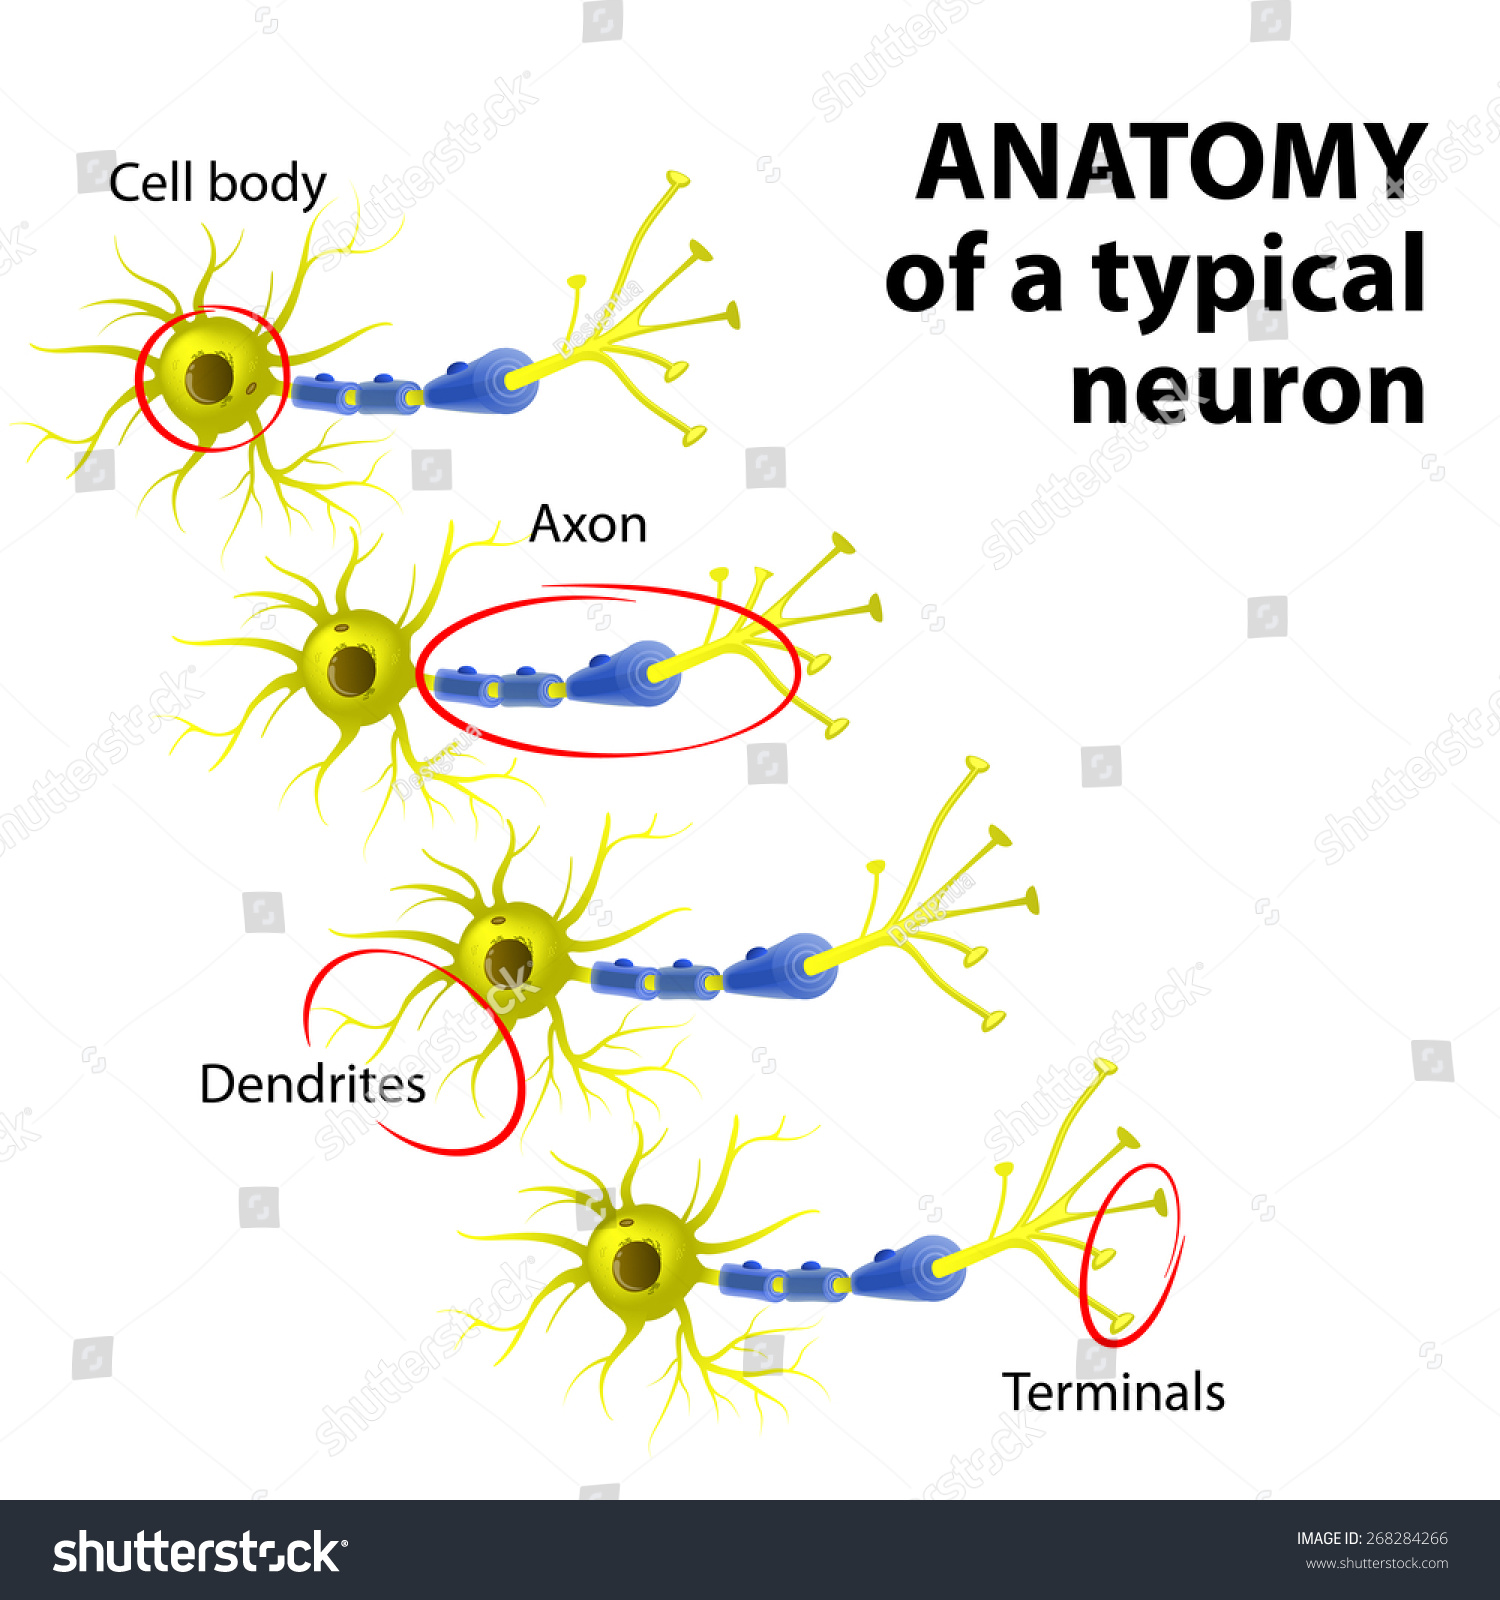
\includegraphics[width=0.5\textwidth]{chap2/figure/neuron.jpg}
    \caption{Structure of neuron \cite{shutterstock_neuron_anatomy}.}
    \label{fig:neuron}
\end{figure}


\subsection{Neural Code.}
The neural code refers to the mechanisms by which the human brain represents and processes information, a topic that remains a central and unresolved challenge in neuroscience \cite{shimazaki2025neural, cao2025neuronal, tee2018information}. Despite decades of research, it is widely accepted that neural information encoding relies on three key principles: spikes, sparsity, and static suppression. First, neurons communicate primarily through the generation and propagation of action potentials, or spikes, which are all-or-none events that encode information in their timing and occurrence rather than their amplitude \cite{shimazaki2025neural, tee2018information}. This discrete, event-based signaling is fundamentally different from the continuous-valued representations used in conventional \glspl{ann}, and recent engineering analyses suggest that discrete coding is essential for reliable information transmission in the brain \cite{tee2018information}. Second, neural activity is characteristically sparse, with most neurons remaining quiescent for extended periods and only a small subset active at any given time, a property that enhances memory efficiency and computational power \cite{cao2025neuronal, fernandino2022decoding}. Third, static suppression mechanisms in sensory systems enable neurons to preferentially respond to dynamic, changing stimuli while filtering out static or redundant information, thereby optimizing sensory processing \cite{shimazaki2025neural}. In terms of computational models, both \glspl{ann} and \glspl{snn} can address similar tasks, but their neuron models differ fundamentally. \glspl{ann} compute a weighted sum of inputs and apply a nonlinear activation function such as ReLU, resulting in continuous-valued outputs. In contrast, SNNs accumulate weighted input spikes to a membrane potential, and a spike is emitted only when this potential crosses a threshold, making the output inherently event-driven and temporally precise \cite{shimazaki2025neural, tee2018information}. This distinction underpins the efficiency and biological plausibility of SNNs for modeling real neural computation. The Figure \ref{fig:neuron} shows the anatomy of a biological neuron.

\subsection{Neuron Model.}
\glspl{ann} and \glspl{snn} are both capable of addressing similar computational tasks, but they differ fundamentally in their neuron models. In ANNs, each neuron computes a weighted sum of its inputs and passes this value through a non-linear activation function, such as the \gls{relu}, to produce its output. This approach enables efficient gradient-based learning and is well-suited for static data representations \cite{Xu2024}.

In contrast, SNNs employ a more biologically inspired neuron model. Here, the weighted sum of inputs contributes to the neuron's membrane potential $U(t)$. When this potential reaches a defined threshold $\theta$, the neuron emits a spike, transmitting information to subsequent neurons. Inputs to SNNs are typically spikes that arrive at different time instants, and the neuron's output is event-driven rather than continuous. This mechanism allows SNNs to process temporal and event-based data efficiently, often resulting in lower energy consumption and more realistic neuronal dynamics \cite{Lin2024}.

While both ANN and SNN architectures can achieve comparable performance on certain tasks, SNNs offer advantages in terms of energy efficiency and biological plausibility, especially for event-driven applications. However, training SNNs remains challenging due to the non-differentiable nature of spike generation, requiring specialized learning algorithms.


\subsection{Encoding and Decoding Spikes in Spiking Neural Networks}

\glspl{snn} process information using discrete spikes, inspired by biological neural systems. A central challenge is how to encode input data as spike trains and how to decode spike outputs for interpretation. Recent research has advanced both encoding and decoding strategies, optimizing SNNs for efficiency and accuracy \cite{Zhou2024}.

\textbf{Input Encoding:}  
Three principal encoding schemes are widely used:
\begin{itemize}
    \item \textit{Rate Coding:} The intensity of the input is represented by the firing rate or spike count within a time window. Higher input values yield more spikes. This method is robust but can require longer time windows for accurate representation \cite{Zhou2024}.
    \item \textit{Temporal (Latency) Coding:} Information is encoded in the timing of spikes, such as the time-to-first-spike (TTFS) approach, where stronger inputs cause earlier spikes. This enables rapid and energy-efficient computation, as fewer spikes are needed \cite{Gu2024}.
    \item \textit{Delta/Change Coding:} Spikes are generated only when there is a change in input intensity, capturing dynamic features and reducing redundancy. This is particularly effective for event-based sensors like Dynamic Vision Sensors (DVS) and silicon cochleas, which directly produce spike streams in response to environmental changes \cite{Baek2024}.
\end{itemize}

\textbf{Output Decoding:}  
To interpret SNN outputs, several decoding strategies are employed:
\begin{itemize}
    \item \textit{Rate Decoding:} The predicted class is assigned to the neuron with the highest firing rate.
    \item \textit{Latency Decoding:} The class is determined by the neuron that fires first.
    \item \textit{Population Coding:} Aggregates information from multiple neurons, overcoming the limitations of individual firing rates and enabling more robust and rapid processing.
\end{itemize}

Recent benchmarking studies have compared these encoding and decoding methods, highlighting trade-offs between speed, accuracy, and energy efficiency. For example, time-to-first-spike coding can achieve high accuracy with minimal spikes, while rate coding offers greater error tolerance and is more compatible with backpropagation-based training \cite{Zhou2024, Gu2024}.
